\section{Feature extraction}

To improve the performance of the models that we want to train, we will explore some transformations of the initial dataset. We do that by extracting subsets of the variables, by applying transformations to them, by remove the variables that show more correlation or by creating a new dataset based on a principal components analysis.

\subsection{Intuitive transformations}

After the exploratory data analysis of section 1, we feel that transforming some variables with functions and trying different combinations can have an impact in terms of make the underlying structure of the data more accessible.

\textbf{Logs}

In the exploratory analysis we saw that applying the logarithm to some variables greatly changes they aspect when ploting them with the price target variable. We then decide to apply logarithms to some of the variables: bathrooms, bedrooms, sqft\_living, floors, sqft\_lot.



\textbf{Ratios}\\
While exploring the variables in our dataset we had the intuition about the ratio relationship between some variables. For example, the ratio between number of bedrooms to number of bathroom may be a good feature to help us predict the house price. Exploring on the Tax policy in USA\cite{tax}, we learn that tax of house also base on the characteristics of the house. Therefore we though it will be useful to check those features. We created new features based on ratios of pairs of the following list of variables from the dataset: bathrooms, bedrooms, sqft\_living, floors, sqft\_lot, logbathrooms, logbedrooms, logsqft\_living.


%"bathrooms.bedrooms.ratio"   "bedrooms.sqft.living.ratio" "bathroom.sqft.living.ratio" "sqft.ratio" "floor.sqft.living.ratio"   "floor.sqft.lot.ratio" "floor.bedrooms.ratio"       "floor.bathrooms.ratio"      "sqft.living.floors.ratio"  "bedrooms.floors.ratio"    



\subsection{Correlation}

Finally, we inspect different groups of variables to see which of them are highly correlated (a correlation greater than 0.7). We know a many machine learning models suffer from being trained over highly correlated variables. So we create new datasets based on subsets of features that are not highly correlated.

\begin{figure}[H]
    \centering
        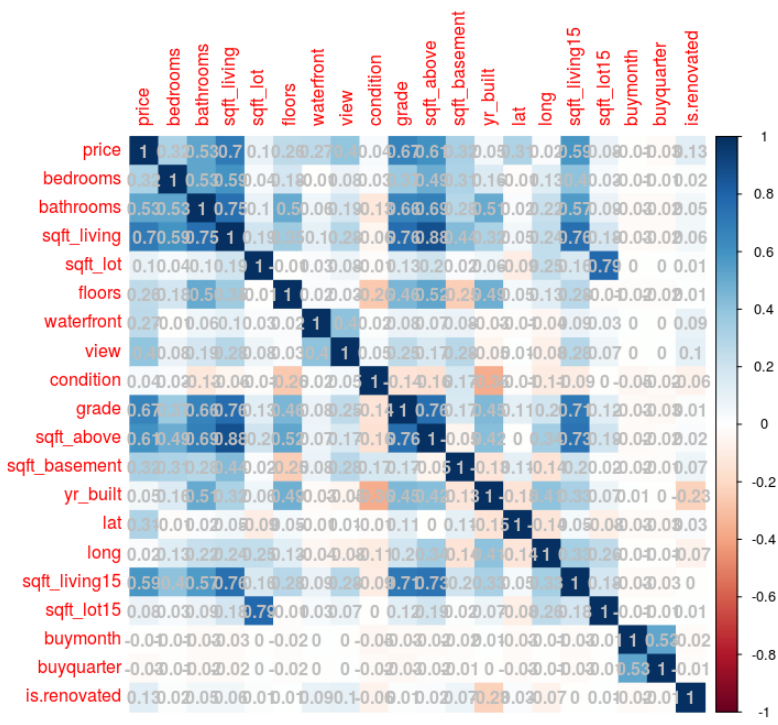
\includegraphics[width=0.8\textwidth]{img/corr01.png}
    \caption{Correlation matrix of a subset of tha continuous variables of the original dataset }\label{fig:rf_sfs}
\end{figure}
% plots

Based on that, we built 4 different subsets of features, where in each of them we will make sure that no pair of variables has a correlation higher than 0.7 or lower than -0.7. Two sets contain only different subsets of the original continuous variables with high correlations removed. Then a third subset contains logarithimic transformations with high correlations removed. Finally a fourth dataset contains ratio variables with high correlations removed. In each of them we remove one of the variables that is highly correlated with another one.

% lsit of subsets


\subsection{PCA}

